
% Introduce detector, location, basic info (e.g., chamber count)
% What is the technology
% Anatomy of a chamber
% How are they arranged in the barrel/endcap
% Coverage
% What do they measure
% Precision
% Performance

Located in the MB are 250 Drift Tube (DT) chambers, layered between RPCs, and arranged to provide coverage within $|\eta|<1.2$ overlapping with the CSC coverage in the muon endcaps (see Fig.~\ref{fig:DT}). DT chambers are labeled by MB station n, then by wheel w, like ``MBn$\pm$w.'' A single DT consists of a long aluminum drift cell filled with a gas mixture of 85~\% Ar and 15~\% CO2 and a central anode wire strung length-wise inside the cell held at \SI{+3600}{V}. Electrode strips held at \SI{+1800}{V} and cathode strips held at \SI{-1200}{V} line the walls of each cell and help shape the electric field inside (see the diagram in Fig.~\ref{fig:DTDiagram}). In MB1-MB3, the DT chambers are grouped into three collections of four consecutive, stagered layers of drift tubes called Super Layers (SLs), while in MB4 there are only two SLs per chamber. The inner-most and outer-most SL in a DT chamber measure $r$-$\phi$ coordinates in the bending plane, while the middle SL measures along the $z$-coordinate. Between the outer-most and middle SL is a honeycomb layer that produces a $\SI{28}{cm}$ separation of measurements in the bending plane, which aid in determining muon track bending. In MB4, DT chambers consist only of the two SLs measuring the $r$-$\phi$-coordinate, with no honeycomb spacer or $z$-coordinate SL. The spatial resolution per cell is at least \SI{250}{\micro\meter}, corresponding to a roughly \SI{100}{\micro\meter} resolution per chamber, while the time resolution per DT chamber is \SI{2}{ns}.

\begin{figure}[H]
    \centering
   { 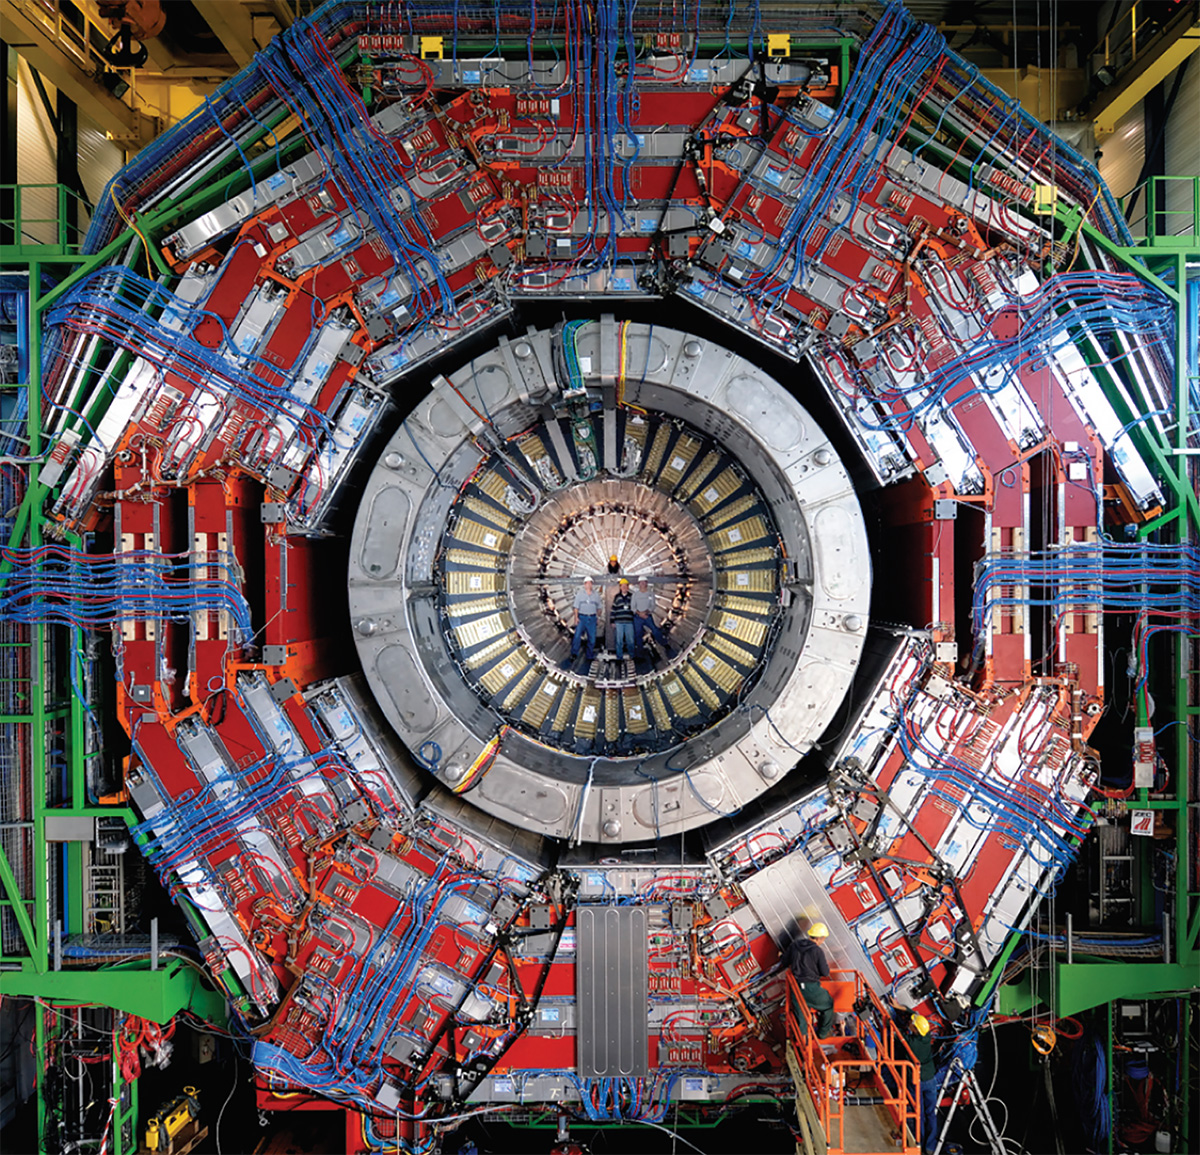
\includegraphics[width=\textwidth]{Images/CMS/DT.jpg}}
    \caption{A photograph of DT chambers (silver boxes) installed in the return yoke (red structure) of a wheel in the muon barrel.}
    \label{fig:DT}
\end{figure}

\begin{figure}[H]
    \centering
    {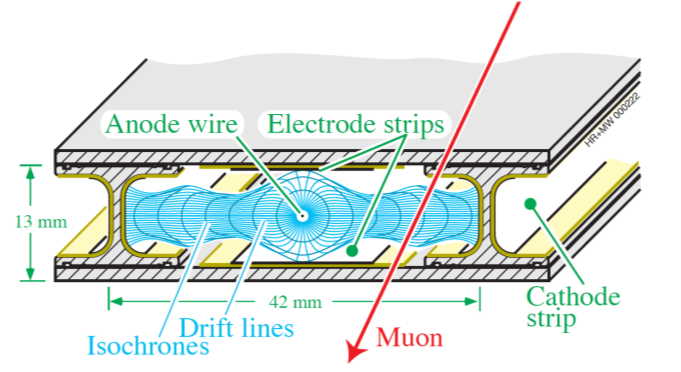
\includegraphics[width=1\textwidth]{Images/CMS/DTDiagram.png}}
    \caption{A diagram of a single DT chamber.}
    \label{fig:DTDiagram}
\end{figure}